%	第二章学习开始
%	字符 babel宏包

\documentclass[UTF8]{ctexart}
\usepackage{graphicx}	% 插入图片的宏包
\usepackage{subfigure}
\graphicspath{{figs/}}

\usepackage{ctex}
\begin{document}
%	,.:;!? 标点后应该加空格 
%	单引号与双引号之间用  \, 隔开
%	- 号 单用连字符 两个用是en dash,表数字范围  三个用是em dash,表示破折号
%	省略号用\dots或者\ldots
%	~是带子	#是宏定义	$是数学模式	%是注释符	
%	&是表格对齐	{}是分组	_是数学下标	\是宏命令
\begin{figure}[ht]
	\centering
	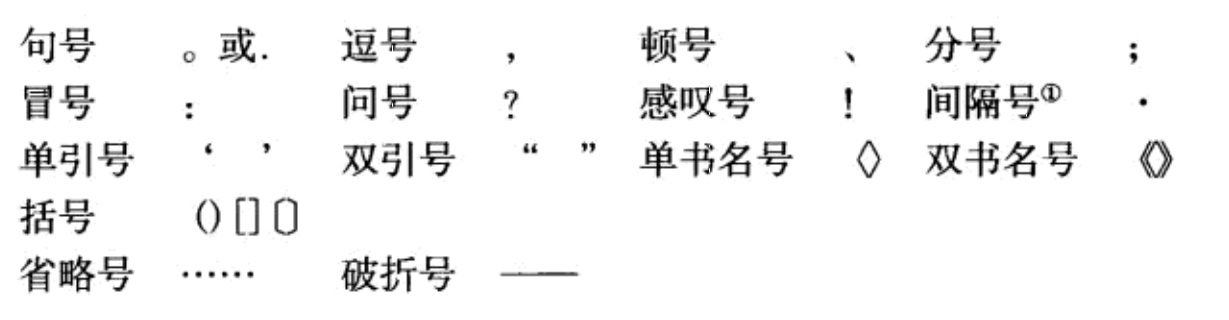
\includegraphics[scale=0.5]{中文符号.jpg}
	\caption{中文字符包}		% 插入编号标题
	\label{fig:ope}	% 定义标签,方便引用	
\end{figure}

%	中文标点由xeCJK宏包决定,默认全角字符,可以使用\punctstyle
%	空格与换行,'\ '可以在宏命令后边加空格,	~为带子,禁止在这种空格分行,用于表示不可分割的情况
happy \TeX ing ,happy \TeX\ ing
1~2

%	西文的符号后应该加空格,否则无法换行,大写字母后为缩写,小写后为句末,必须使用“\ ”或者“\@.”来指明是大写字母后句末。
A cbsvbu. Absivsb.

U.S.A. means.

AA\ huiorheveuAA\@.

%	有时候需要把汉字与其他内容连接时的空格去除,使用\mbox{text}
\mbox{不是吧}-a 不同于条目-b
%	还有时候需要全局禁用汉字与其他字符的空格,使用\CJKsetecglue

%	幻影,同字符占位\hphantom和\vphantom
啦啦啦嘿嘿嘿

啦啦\phantom{啦嘿}嘿嘿

%	分段,两个换行
%	命令或环境变量内部换行使用\par
%	除了分段,还可以直接另起一行:“\\”用于诗歌和“\linebreak”
%	但是正常行文中不会使用
%	\\可以带一个可选长度的参数 \\{}
这是一句话,\\这又是一句话。

这是一句话,\linebreak 这又是一句话。

% \symbol{n}可以直接用在字体库的编码来输入符号
\symbol{"DE"}

%	字体属性:1.字号(font size)	2.字体编码(font encoding)	3.字体族(font family)	4.字体形状(font shape)	5.字体系列(font series)


%	修改字号字体
\begin{figure}[ht]
	\centering
	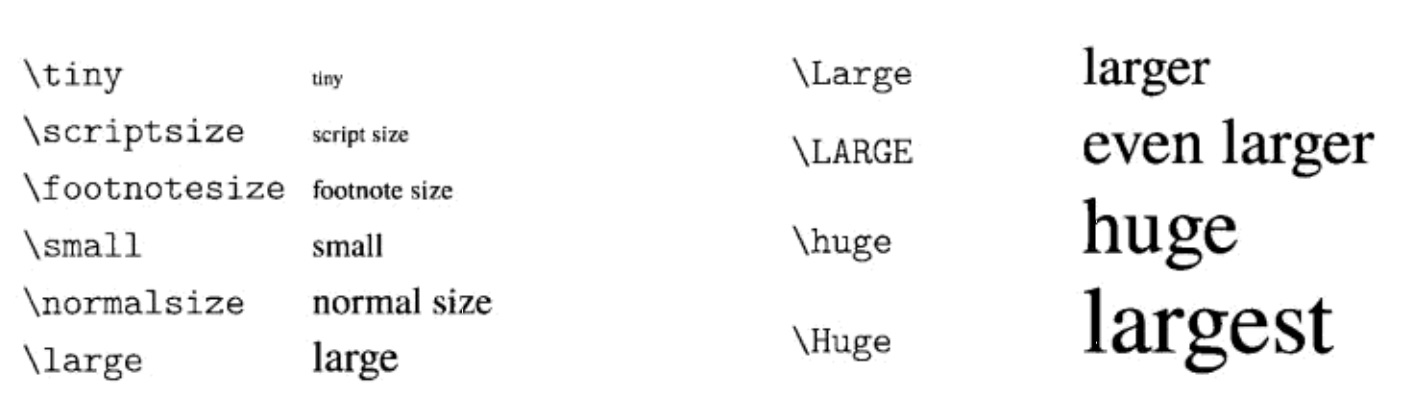
\includegraphics[scale=0.5]{修改字号.jpg}
	\caption{修改字号}		% 插入编号标题
	\label{fig:ope1}	% 定义标签,方便引用	
\end{figure}





\end{document}